%Рефракція
{
\psset{linestyle=none}
\textcolor{white}{\Large Refraction}

\begin{itemize}
\item Рефракція ЕМВ залежить від довжини хвилі, як це видно з прикладу призми нижче.
\end{itemize}

\begin{tabular}{cl}
%Prism
\begin{minipage}[b]{1.8in}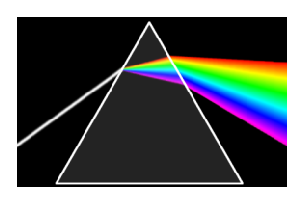
\includegraphics{pictures/prism.eps}
\end{minipage}&
\hspace{0.0in}
\begin{minipage}[b]{1.8in}\textcolor{white}{%
	Використовуючи скляну призму, біле світло може бути розділено заломленням у спектр його складових кольорів. Усі довжини хвиль ЕМВ можуть бути заломлені, використовуючи відповідні матеріали. Не всі скляні призми поводяться однаково; прямокутна призма буде діяти як дзеркало, а не легкий рефрактор. Критичний кут справжньої світлопереломної призми - це 42\degree.
	}
\end{minipage}
\vspace{0.3in}\\
%
%Convex
\vspace{0.3in}
\psframebox{
	\psset{linestyle=solid,fillstyle=solid,fillcolor=gray}
	\psarc{c-c}(+.693,0){.8}{150}{210}
	\psarc{c-c}(-.693,0){.8}{330}{30}
	\rput(-.6,0){Source}
	\rput(.5,.2){Focal point}
	\psset{linestyle=solid,fillstyle=none}
	\psline(-.4,+.207)(-0.08,+.207)(.086,+.180)(.6,-.1)
	\psline(-.4,-.207)(-0.08,-.207)(.086,-.180)(.6,+.1)
}&
\hspace{0.0in}
\begin{minipage}[b]{1.8in}\textcolor{white}{%
	Випуклі лінзи роблять об'єкти зближеними та використовуються для корекції далекоглядності.}
\end{minipage}
\vspace{0.3in}\\
%
%Concave
\vspace{0.3in}
\psframebox{
	\psclip{\psframe[fillstyle=none,linestyle=none,linearc=0,framearc=0](-.157,-.4)(.157,.4)}
	\psframe[fillstyle=solid,fillcolor=gray,linestyle=none,linearc=0,framearc=0](-.15,-.4)(.15,.4)
	\psset{linestyle=solid,fillstyle=solid,fillcolor=Black}
	\pscircle(+.85,0){.8}
	\pscircle(-.85,0){.8}
	\psline(-.157,-.389)(+.157,-.389)
	\psline(-.157,+.389)(+.157,+.389)
	\endpsclip
	\rput(-.6,0){\white Source}
	\psset{linestyle=solid,fillstyle=none}
	\psline(-.4,+.180)(-0.086,+.180)(.08,+.207)(.6,+.4)
	\psline(-.4,-.180)(-0.086,-.180)(.08,-.207)(.6,-.4)
}&
\hspace{0.0in}
\begin{minipage}[b]{1.8in}\textcolor{white}{%
	Вбудовані лінзи роблять об'єкти далеко видно і використовуються для виправлення ближнього сприйняття.}
\end{minipage}
\vspace{0.3in}\\
%
%
%Gravity lens
\vspace{0.0in}
\psframebox{
%	\rput(-.75,0){
%		\PstStarFive[unit=.1,
%			fillstyle=solid,
%			fillcolor=white,
%			linestyle=solid,
%			linecolor=white,
%			PolyIntermediatePoint=0.3,
%			PolyRotation=45]
%	}
%	\pscircle[linestyle=solid,
%		linecolor=white,
%		fillstyle=solid,
%		fillcolor=Black](0,-.1){.2}
%	\pscurve[linestyle=solid,linecolor=white,fillstyle=none](-.6,.05)(0,+.15)(.6,.05)
%	\rput(.85,0){
%		\psclip{\psline[fillstyle=none,linestyle=solid,linecolor=white,linearc=0](.3;150)(0,0)(.3;210)}
%			\psclip{\pscircle[linestyle=solid,linecolor=white,fillstyle=solid,fillcolor=white]{.2}}% Eyeball
%			\rput(-.2,0){
%				\pscircle[fillstyle=solid,fillcolor=gray]{.10}% Iris
%				\pscircle[fillstyle=solid,fillcolor=Black]{.05}% Pupil
%			}
%			\endpsclip
%		\endpsclip
%	}
%http://imgsrc.hubblesite.org/hu/db/2004/08/images/a/formats/large_web.jpg
	\rput[tl]{90}(-0.15,0){\textcolor{gray}{Photo by STScI}}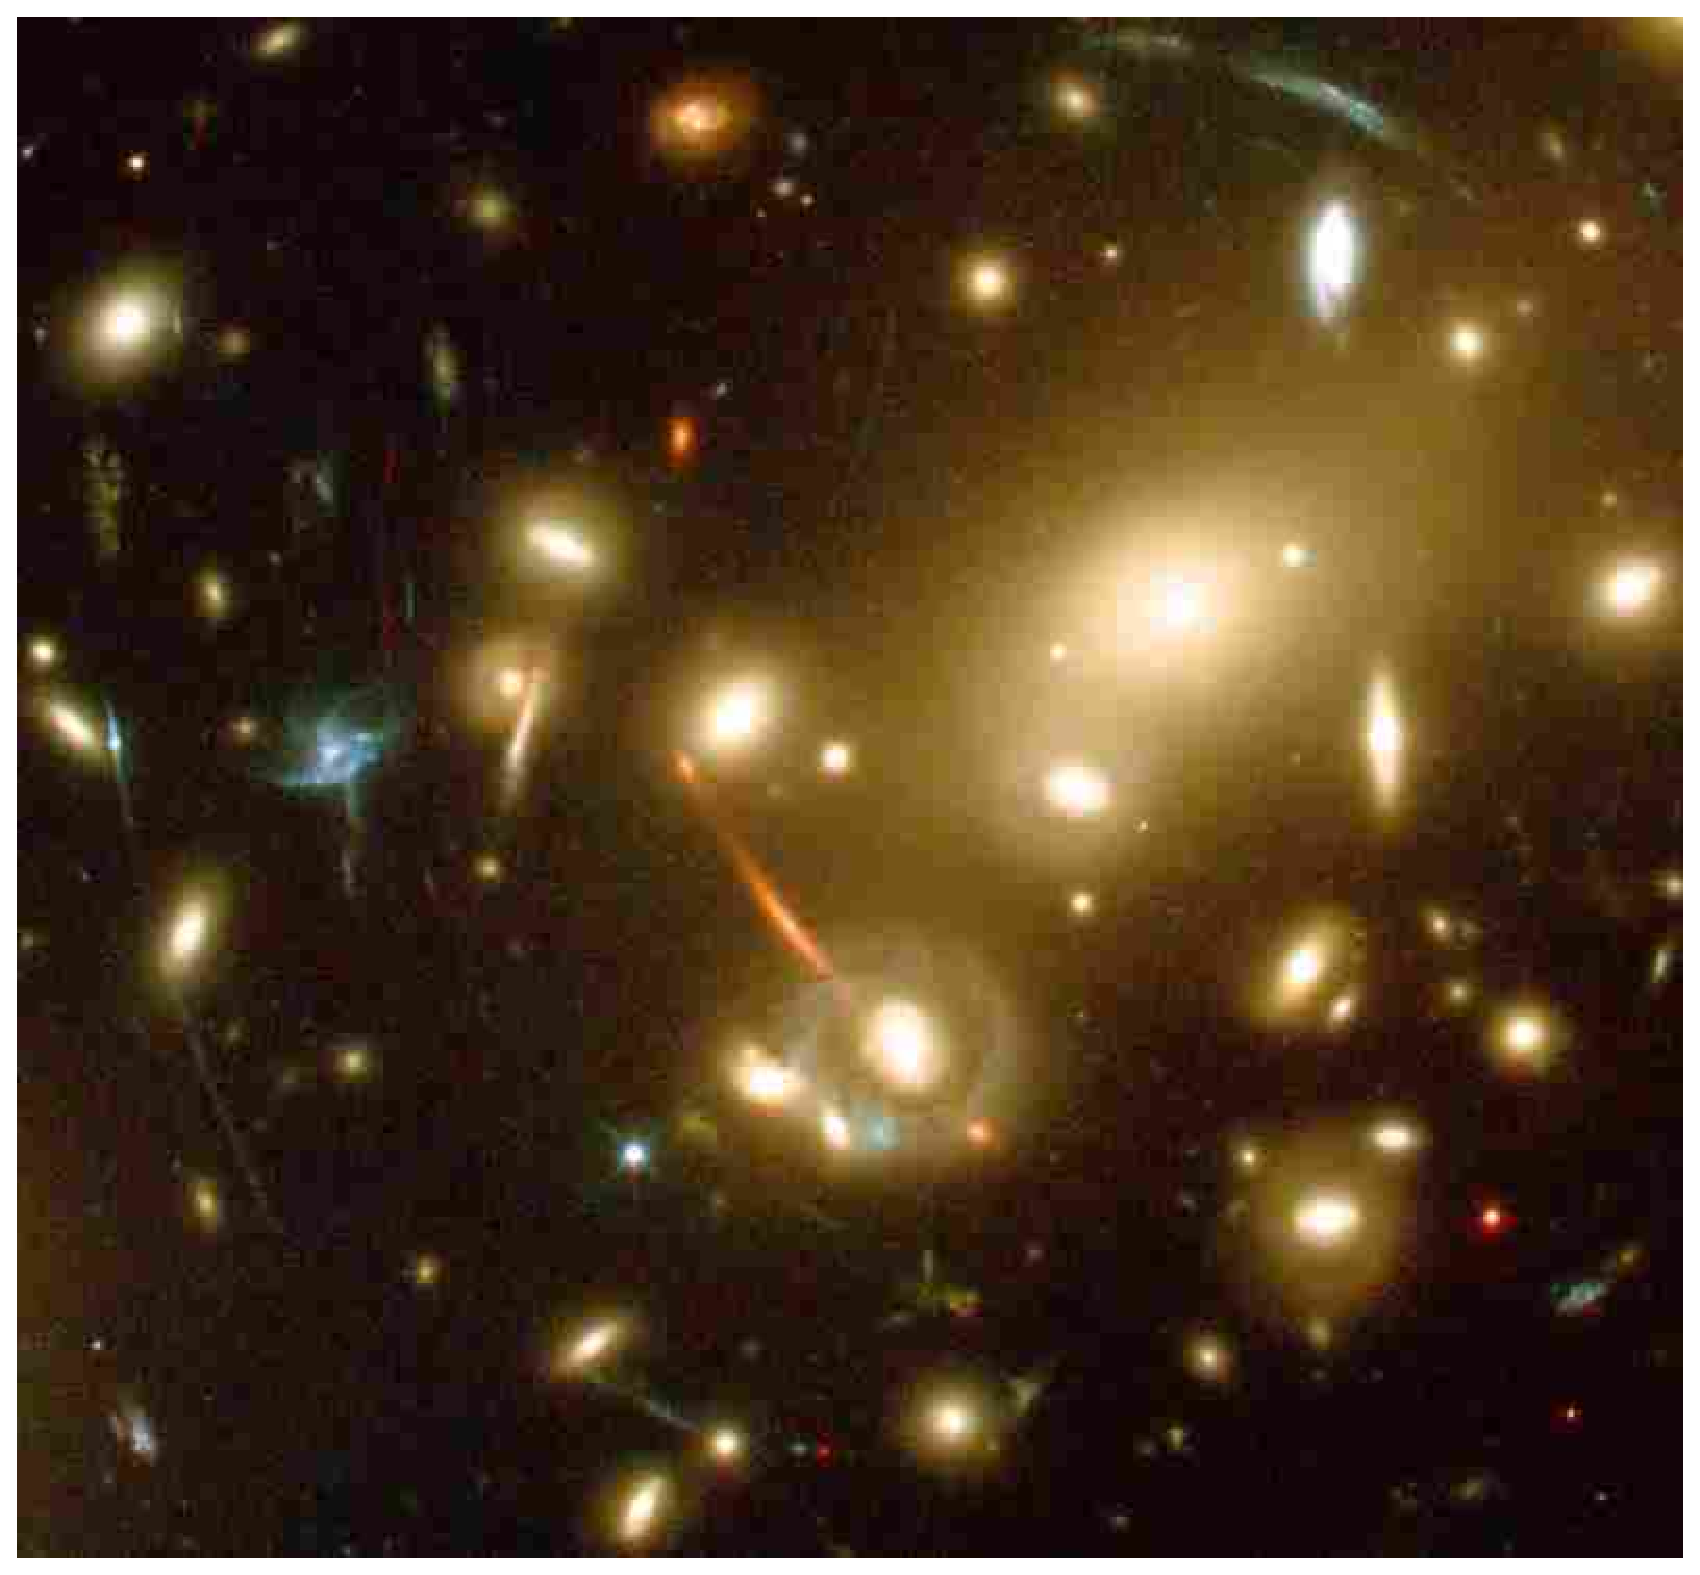
\includegraphics[width=1in]{pictures/gravlens.eps}
}&
\begin{minipage}[b]{1.8in}\textcolor{white}{%
	Важкі предмети, такі як щільні галактики і великі планети, змушують світло згинатися під впливом гравітаційної лінзи.\vspace{0.2in}}
\end{minipage}
\vspace{0.0in}\\
%
\end{tabular}
}
